% 2-15-rb-tree.tex

%%%%%%%%%%%%%%%%%%%%
\documentclass[a4paper, justified]{tufte-handout}

% hw-preamble.tex

% geometry for A4 paper
% See https://tex.stackexchange.com/a/119912/23098
\geometry{
  left=20.0mm,
  top=20.0mm,
  bottom=20.0mm,
  textwidth=130mm, % main text block
  marginparsep=5.0mm, % gutter between main text block and margin notes
  marginparwidth=50.0mm % width of margin notes
}

% for colors
\usepackage{xcolor} % usage: \color{red}{text}
% predefined colors
\newcommand{\red}[1]{\textcolor{red}{#1}} % usage: \red{text}
\newcommand{\blue}[1]{\textcolor{blue}{#1}}
\newcommand{\teal}[1]{\textcolor{teal}{#1}}

\usepackage{todonotes}

% heading
\usepackage{sectsty}
\setcounter{secnumdepth}{2}
\allsectionsfont{\centering\huge\rmfamily}

% for Chinese
\usepackage{xeCJK}
\usepackage{zhnumber}
\setCJKmainfont[BoldFont=FandolSong-Bold.otf]{FandolSong-Regular.otf}

% for fonts
\usepackage{fontspec}
\newcommand{\song}{\CJKfamily{song}} 
\newcommand{\kai}{\CJKfamily{kai}} 

% To fix the ``MakeTextLowerCase'' bug:
% See https://github.com/Tufte-LaTeX/tufte-latex/issues/64#issuecomment-78572017
% Set up the spacing using fontspec features
\renewcommand\allcapsspacing[1]{{\addfontfeature{LetterSpace=15}#1}}
\renewcommand\smallcapsspacing[1]{{\addfontfeature{LetterSpace=10}#1}}

% for url
\usepackage{hyperref}
\hypersetup{colorlinks = true, 
  linkcolor = teal,
  urlcolor  = teal,
  citecolor = blue,
  anchorcolor = blue}

\newcommand{\me}[4]{
    \author{
      {\bfseries 姓名:}\underline{#1}\hspace{2em}
      {\bfseries 学号:}\underline{#2}\hspace{2em}\\[10pt]
      {\bfseries 评分:}\underline{#3\hspace{3em}}\hspace{2em}
      {\bfseries 评阅:}\underline{#4\hspace{3em}}
  }
}

% Please ALWAYS Keep This.
\newcommand{\noplagiarism}{
  \begin{center}
    \fbox{\begin{tabular}{@{}c@{}}
      请独立完成作业,不得抄袭。\\
      若得到他人帮助, 请致谢。\\
      若参考了其它资料,请给出引用。\\
      鼓励讨论,但需独立书写解题过程。
    \end{tabular}}
  \end{center}
}

\newcommand{\goal}[1]{
  \begin{center}{\fcolorbox{blue}{yellow!60}{\parbox{0.50\textwidth}{\large 
    \begin{itemize}
      \item 体会``思维的乐趣''
      \item 初步了解递归与数学归纳法 
      \item 初步接触算法概念与问题下界概念
    \end{itemize}}}}
  \end{center}
}

% Each hw consists of four parts:
\newcommand{\beginrequired}{\hspace{5em}\section{作业 (必做部分)}}
\newcommand{\beginoptional}{\section{作业 (选做部分)}}
\newcommand{\beginot}{\section{Open Topics}}
\newcommand{\begincorrection}{\section{订正}}
\newcommand{\beginfb}{\section{反馈}}

% for math
\usepackage{amsmath, mathtools, amsfonts, amssymb}
\newcommand{\set}[1]{\{#1\}}

% define theorem-like environments
\usepackage[amsmath, thmmarks]{ntheorem}

\theoremstyle{break}
\theorempreskip{2.0\topsep}
\theorembodyfont{\song}
\theoremseparator{}
\newtheorem{problem}{题目}[subsection]
\renewcommand{\theproblem}{\arabic{problem}}
\newtheorem{ot}{Open Topics}

\theorempreskip{3.0\topsep}
\theoremheaderfont{\kai\bfseries}
\theoremseparator{:}
\theorempostwork{\bigskip\hrule}
\newtheorem*{solution}{解答}
\theorempostwork{\bigskip\hrule}
\newtheorem*{revision}{订正}

\theoremstyle{plain}
\newtheorem*{cause}{错因分析}
\newtheorem*{remark}{注}

\theoremstyle{break}
\theorempostwork{\bigskip\hrule}
\theoremsymbol{\ensuremath{\Box}}
\newtheorem*{proof}{证明}

% \newcommand{\ot}{\blue{\bf [OT]}}

% for figs
\renewcommand\figurename{图}
\renewcommand\tablename{表}

% for fig without caption: #1: width/size; #2: fig file
\newcommand{\fig}[2]{
  \begin{figure}[htbp]
    \centering
    \includegraphics[#1]{#2}
  \end{figure}
}
% for fig with caption: #1: width/size; #2: fig file; #3: caption
\newcommand{\figcap}[3]{
  \begin{figure}[htbp]
    \centering
    \includegraphics[#1]{#2}
    \caption{#3}
  \end{figure}
}
% for fig with both caption and label: #1: width/size; #2: fig file; #3: caption; #4: label
\newcommand{\figcaplbl}[4]{
  \begin{figure}[htbp]
    \centering
    \includegraphics[#1]{#2}
    \caption{#3}
    \label{#4}
  \end{figure}
}
% for margin fig without caption: #1: width/size; #2: fig file
\newcommand{\mfig}[2]{
  \begin{marginfigure}
    \centering
    \includegraphics[#1]{#2}
  \end{marginfigure}
}
% for margin fig with caption: #1: width/size; #2: fig file; #3: caption
\newcommand{\mfigcap}[3]{
  \begin{marginfigure}
    \centering
    \includegraphics[#1]{#2}
    \caption{#3}
  \end{marginfigure}
}

\usepackage{fancyvrb}

% for algorithms
\usepackage[]{algorithm}
\usepackage[]{algpseudocode} % noend
% See [Adjust the indentation whithin the algorithmicx-package when a line is broken](https://tex.stackexchange.com/a/68540/23098)
\newcommand{\algparbox}[1]{\parbox[t]{\dimexpr\linewidth-\algorithmicindent}{#1\strut}}
\newcommand{\hStatex}[0]{\vspace{5pt}}
\makeatletter
\newlength{\trianglerightwidth}
\settowidth{\trianglerightwidth}{$\triangleright$~}
\algnewcommand{\LineComment}[1]{\Statex \hskip\ALG@thistlm \(\triangleright\) #1}
\algnewcommand{\LineCommentCont}[1]{\Statex \hskip\ALG@thistlm%
  \parbox[t]{\dimexpr\linewidth-\ALG@thistlm}{\hangindent=\trianglerightwidth \hangafter=1 \strut$\triangleright$ #1\strut}}
\makeatother

% for footnote/marginnote
% see https://tex.stackexchange.com/a/133265/23098
\usepackage{tikz}
\newcommand{\circled}[1]{%
  \tikz[baseline=(char.base)]
  \node [draw, circle, inner sep = 0.5pt, font = \tiny, minimum size = 8pt] (char) {#1};
}
\renewcommand\thefootnote{\protect\circled{\arabic{footnote}}} % feel free to modify this file
%%%%%%%%%%%%%%%%%%%%
\title{第3-10讲: 图的连通性}
\me{林凡琪}{211240042}{}{}
\date{\zhtoday} % or like 2019年9月13日
%%%%%%%%%%%%%%%%%%%%
\begin{document}
\maketitle
%%%%%%%%%%%%%%%%%%%%
\noplagiarism % always keep this line
%%%%%%%%%%%%%%%%%%%%
\begin{abstract}
  % \begin{center}{\fcolorbox{blue}{yellow!60}{\parbox{0.65\textwidth}{\large 
  %   \begin{itemize}
  %     \item 
  %   \end{itemize}}}}
  % \end{center}
\end{abstract}
%%%%%%%%%%%%%%%%%%%%
\beginrequired

%%%%%%%%%%%%%%%
\begin{problem}[CZ 5.4]
证明:若v是图G的割点,则$v$一定不是$G^-$的各点
\end{problem}

\begin{solution}
  For the node $u$ that is different from $v$, $w$\\
  If there are different connected branches of $G-v$, it means that the $(u,w)$ edge does not exist in $G$, so there is the $(u,v)$ edge in $\overline{G}$. So in $\overline{G}$, there is a pathway between $u$ and $w$ that does not go through $v$. \\
  If in the same connected branch of $G-v$, for a point $p$ of another connected branch, there are no two edges in $G$ $(u,p)$ and $(w,p)$, so there are two edges in $\overline{G}$. So in $\overline{G}$, there is a pathway between $u$ and $w$ that does not go through $v$. \\
  In summary, there is a path between any two points $u$ and $w$ in $\overline{G}$ that are different from $v$. Therefore, $v$ is not a cut point.
\end{solution}
%%%%%%%%%%%%%%%

%%%%%%%%%%%%%%%
\begin{problem}[CZ 5.8]
(a)设G是非平凡的连通图.证明:若v是G的生成树的一个端点,则v不是G的
割点.\\
(b)利用(a)的结论给出下面事实的另一种证明:任意一个非平凡的连通图至少包含
两个不是割点的顶点.\\
(c) 设v是非平凡连通图G的一个顶点证明:存在G的一个生成树,它包含G中
所有与v相关联的边.\\
(d)证明:若连通图G恰有两个非割点的顶点,则G是一条路.[提示:若树T包含
一个度大于2的顶点,则T包含两个以上的端点]

\end{problem}

\begin{solution}
  (a)
  In the spanning tree $T$ of $G$ , the theorem shows that its endpoint has a degree of 1 , not a cut point.\\
  In the process of reducing from $T$ to $G$, it is a process of continuous edges, and the connectivity of the graph is enhanced. If a point is not a cut point in $T$, it must not be a cut point in $G$. \\
  (b)
  The spanning tree of any nontrivial graph contains at least two endpoints , and it can be seen from $( a) $ that these two endpoints must not be cut points in the original nontrivial graph , so the number of cut points is at least 2. \\
  (c)
  For any spanning tree $T$ of $G$, if there is an edge associated with $v$ in $G$ that is not in $T$, add $T$ to that edge, and delete an edge in the resulting ring where neither endpoint is $v$. \\
  After this operation, the built graph is still a spanning tree of $G$. \\Therefore, by continuously constructing through this operation, a tree can be formed that meets the above conditions. \\
  (d)
  From (c) it can be seen that at any point $v$, there is a spanning tree $T$ of $G$, containing all the edges associated with $v$ in $G$.\\
  As can be seen from the hint, none of the vertices in $T$ has a degree of more than 2. \\
  Therefore, all vertices in the figure $G$ do not exceed 2. \\
  Combined with $G$ connectivity and exactly two non-cut endpoints, it is concluded that $G$ is a path.

\end{solution}
%%%%%%%%%%%%%%%

%%%%%%%%%%%%%%%
\begin{problem}[CZ 5.10]
\end{problem}

\begin{solution}
  Assuming that $(u,v)(x,y)$ is not contiguous, then $4$ points are different. Because $G$ is indivisible, any two points are on a ring in the diagram. \\
  If there is a pathway between $u$ and $x$ that does not go through $v$ and $y$, then there must be a pathway between $v$ and $y$ that does not go through $u$ and $x$. At this time, these two pathways and the ring formed by these two edges meet the requirements of the topic. \\
  Otherwise, if there is a path between $u$ and $y$ that does not go through $x$ and $v$, then there must be a path between $x$ and $v$ that does not go through $u$ and $y$. At this time, these two pathways and the ring formed by these two edges meet the requirements of the topic. \\
  Thus there exists a ring satisfying that all four vertices are on that ring.\\
  In summary, these two sides are on a circle.
\end{solution}
%%%%%%%%%%%%%%%

%%%%%%%%%%%%%%%
\begin{problem}[CZ 5.12]
\end{problem}

\begin{solution}
  $1$,$2$\\
  \noindent when k = 1:\\
  \begin{figure}[htbp]
    \centering
    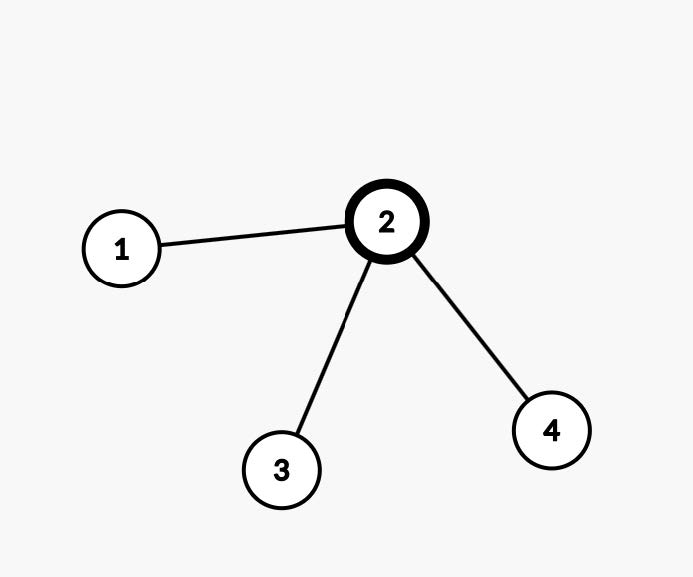
\includegraphics[width = 0.30\linewidth]{figs/b.jpg}
  \end{figure}
  When k = 2:
  \begin{figure}[htbp]
    \centering
    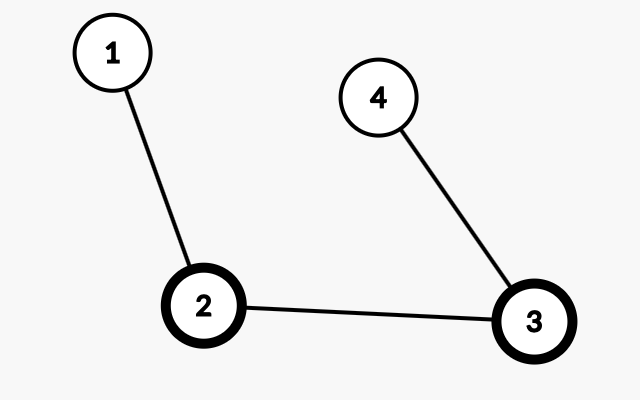
\includegraphics[width = 0.30\linewidth]{figs/c.png}
  \end{figure}

  if$k$>$2$,the number of parts is at least 4. So this assumption is clearly not valid\\
\end{solution}
%%%%%%%%%%%%%%%

%%%%%%%%%%%%%%%
\begin{problem}[CZ 5.18]
\end{problem}

\begin{solution}
  (a)\\
  \begin{figure}[htbp]
    \centering
    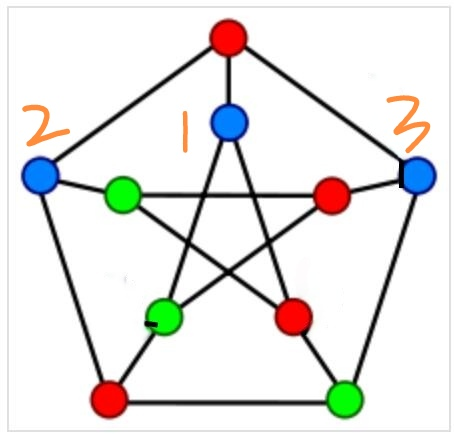
\includegraphics[width = 0.75\linewidth]{figs/d.jpg}
  \end{figure}

  \noindent(b)\\
  \newpage
  \begin{figure}[htbp]
    \centering
    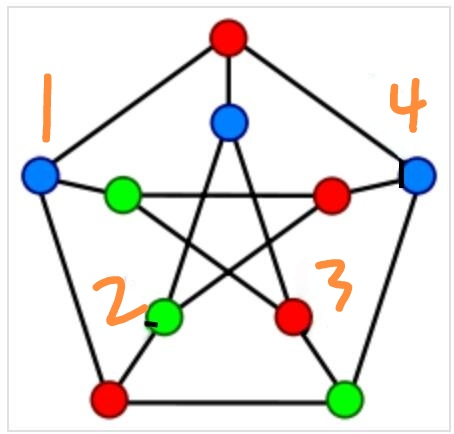
\includegraphics[width = 0.75\linewidth]{figs/e.jpg}
  \end{figure}
\end{solution}
%%%%%%%%%%%%%%%

%%%%%%%%%%%%%%%
\begin{problem}[CZ 5.22]
\end{problem}

\begin{solution}
  (a)
  Proof by contradiction.\\
  Suppose the point connectivity of $G-e$ is p$(p<k-1)$. The connectivity of points with $G$ in the title is at least $k$. \\
  Let $H$ be the plot obtained by removing the smallest set of cut points of graph $G-e$ in $G$. Then in $H$, the edge $e$ is the cut edge. (After removing the side $e$, the figure is not connected). \\
  Then in $H$, you only need to remove one of the two points connected by $e$ to make $H$ unconnected. Therefore, it can be inferred that the connectivity of $G$ is at most $p+1$. \\
  $p+1<k$ from $p<k-1$ is obtained, which contradicts the point connectivity of $G$ at least $k$. Therefore, it is not true.\\
  Therefore, if $G$ is $k$ connected, then $G-e$ is $k-1$ connected\\
  (b)
  Proof by contradiction. \\
  Suppose the edge connectivity of $G-e$ is p$(p<k-1)$. The connectivity of edges with $G$ in the title is at least $k$. \\
  Let the edge cut set of size $p$ in $G-e$ be $S$, then $S+e$ must be a side cut set of $G$. \\
  Therefore, the edge connectivity of $G$ is at most $p+1$\\
  $p+1<k$ from $p<k-1$ is obtained, which contradicts the edge connectivity of $G$ being at least $k$. Therefore, it is not true. \\
  Therefore, if $G$ is $k$ edge-connected, then $G-e$ is $k-1$ edge-connected
\end{solution}
%%%%%%%%%%%%%%%

%%%%%%%%%%%%%%%
\begin{problem}[CZ 5.26]
\end{problem}

\begin{solution}
  Let $S$ be the edge cut set of $G$. Then $G-S$ is divided into $G1, G2$ two maximal connected subgraphs. Assume $|V(G_1)|<|V(G_2)|$, then there is $|V(G_1)|=k<n/2$\\
  Then there are sides from $G_1$ to $G_2$ greater than or equal to $k(\delta(G)-(k-1))$, that is, $\lambda(G) \geq k(\delta(G)-(k-1))$. \\
  From the nature of the quadratic function, the left equation is the smallest when $k=1$, so there is $\lambda(G) \geq \delta(G)$\\
  From the textbook nature $\lambda(G) \leq \delta(G)$, so $\lambda(G) = \delta(G)$
\end{solution}
%%%%%%%%%%%%%%%

%%%%%%%%%%%%%%%
\begin{problem}[CZ 5.34]
\end{problem}

\begin{solution}
  In figure $H$, for any point $u$, $v$ that differs from $w$, there are at least $k$ disjoint $u-v$ paths in figure $G$. Obviously, in the increase point and edge $H$ chart, at least $k$ bars do not intersect $u-v$ paths. \\
  If one of the points is $w$, it is not generally assumed that $u$ is $w$, and it is now necessary to prove that there are $k$ disjoint $u-v$ paths from $v$ to $u$. \\
  Suppose $k$ points in $S$ are $n_1, n_2,...,n_k$. \\
  From $v$ to $n_1$ there are $k$ roads that do not intersect with each other. \\
  Suppose one of them passes $n_i(ineq 1)$, then its and $k-1$ must not pass $n_i$. In summary, there are at least $1$ roads in it, and the point in the $S$ passed through is only $n_1$. \\
  Similarly, for any point $n_i$ in $S$, there is at least one path such that from $v$ to $n_i$ does not pass through the total other points of $S$.
  The path from $v$ to $n_i$, plus the side of $(n_i,w)$, forms the $k$ disjoint $u-v$ path from $v$ to $u$. \\
  In summary, Figure $H$ is $k$ connected.
\end{solution}
%%%%%%%%%%%%%%%

%%%%%%%%%%%%%%%%%%%%
\beginot
%%%%%%%%%%%%%%%
%%%%%%%%%%%%%%%
\begin{ot}[Tarjan's Algorithm]
  [参考资料:\href{https://ieeexplore.ieee.org/document/4569669}{R. Tarjan, "Depth-first search and linear graph algorithms," 12th Annual Symposium on Switching and Automata Theory (swat 1971), East Lansing, MI, USA, 1971, pp. 114-121, doi: 10.1109/SWAT.1971.10.}]

\end{ot}

% \begin{solution}
% \end{solution}
%%%%%%%%%%%%%%%

\begin{ot}[证明 Harary 图是r-连通的]


\end{ot}

% \begin{solution}
% \end{solution}
%%%%%%%%%%%%%%%




% \vspace{0.50cm}
%%%%%%%%%%%%%%%
% \begin{ot}[]
% 
%   \noindent 参考资料:
%   \begin{itemize}
%     \item 
%   \end{itemize}
% \end{ot}

% \begin{solution}
% \end{solution}
%%%%%%%%%%%%%%%

%%%%%%%%%%%%%%%%%%%%
% 如果没有需要订正的题目,可以把这部分删掉

% \begincorrection
%%%%%%%%%%%%%%%%%%%%

%%%%%%%%%%%%%%%%%%%%
% 如果没有反馈,可以把这部分删掉
\beginfb

% 你可以写
% ~\footnote{优先推荐 \href{problemoverflow.top}{ProblemOverflow}}:
% \begin{itemize}
%   \item 对课程及教师的建议与意见
%   \item 教材中不理解的内容
%   \item 希望深入了解的内容
%   \item $\cdots$
% \end{itemize}
%%%%%%%%%%%%%%%%%%%%
% \bibliography{2-5-solving-recurrence}
% \bibliographystyle{plainnat}
%%%%%%%%%%%%%%%%%%%%
\end{document}